\section{Postscript: Reconsidering Divergence Cleaning in \arepo}
\label{sec:c4_postscript}

In Sec. \ref{sec:c4_discussion} we discussed why \arepo\ might be capturing (at least some proxy of) rapid magnetic amplification during the merger when Eulerian simulations of NS mergers at similar resolutions do not.  Since the publication of Ch. \ref{ch:ch4} as \cite{zhu+15}, it has been pointed out that the amplification could be the spurious result of \arepo's divergence cleaning mechanism.

%The MHD equations of motion (Eqn. \ref{eqn:c3_mhd_eqns}) do not contain $\bf{\nabla\cdot B}$, since they are identically zero according to Maxwell's Equations.

In most multidimensional numerical MHD schemes, the ``divergence constraint'' of $\bf{\nabla\cdot B} = 0$ is not guaranteed, and if the implicit divergence terms in Eqn. \ref{eqn:c3_mhd_eqns} are not considered, these schemes can in practice lead to spurious forces and magnetic instabilities \citep{toth00, hopkr16}.  A number of solutions exist (eg. \citealt{toth00}), and the most widely-used is \cite{evanh88}'s constrained transport method, which staggers the different components of the magnetic field within the discretization to maintain the divergence constraint to round-off errors.  This reliance on grid geometry, however, has made it challenging to implement in a moving mesh code \citep{moczvh14}.  Until the recent adoption of constrained transport in \arepo\ in \cite{mocz+16}, the code instead used either the \cite{dedn+02} or \cite{powe+99} divergence control schemes.  The former introduces an additional conserved scalar term $\psi$ to ${\bf U}$ in Eqn. \ref{eqn:c3_mhd_eqns_compact} which is coupled to $\bf{\nabla\cdot B}$ while simultaneously being advected and forced to exponentially decay.  The latter adds a source term to the righthand side of Eqn. \ref{eqn:c3_mhd_eqns_compact} that is proportional to $\bf{\nabla\cdot B}$, which passively advects divergence errors but does not damp them.  The Dedner method is superior because it actively minimizes divergence errors rather than simply preventing their local accumulation, but its implementation in \arepo\ required prohibitively small timesteps and tended to become unstable in highly dynamic environments \citep{pakms13}, hence our use of the Powell scheme.

% DEFENCE NOTE: CT actually keeps the divergence constant, making it only necessary to initialize the simulation with $\bf{\nabla\cdot B} = 0$; see \citealt{toth00}, Sec. 4.1

% DEFENSE NOTE: if the implicit divergence terms in Eqn. \ref{eqn:c3_mhd_eqns} are not considered, these schemes can in practice lead to spurious forces and magnetic instabilities that do not become negligible even at infinite resolution

% DEFENSE NOTE: Pakmor+11 uses the GLM-MHD method, though I find Eqn. 10 of Hopkins and Eqn. 24 of Dedner+02 to be the cleanest representations of this method.  Note that \psi is not proportional to B, but rather just coupled to it - see Eqn. 5 of Dedner, and the explanation around Eqn. 18, which shows that \psi in general has parabolic and hyperbolic (exponentially decreasing) components, leading to both exponential damping as well as transport via waves.

\begin{figure}
\centering
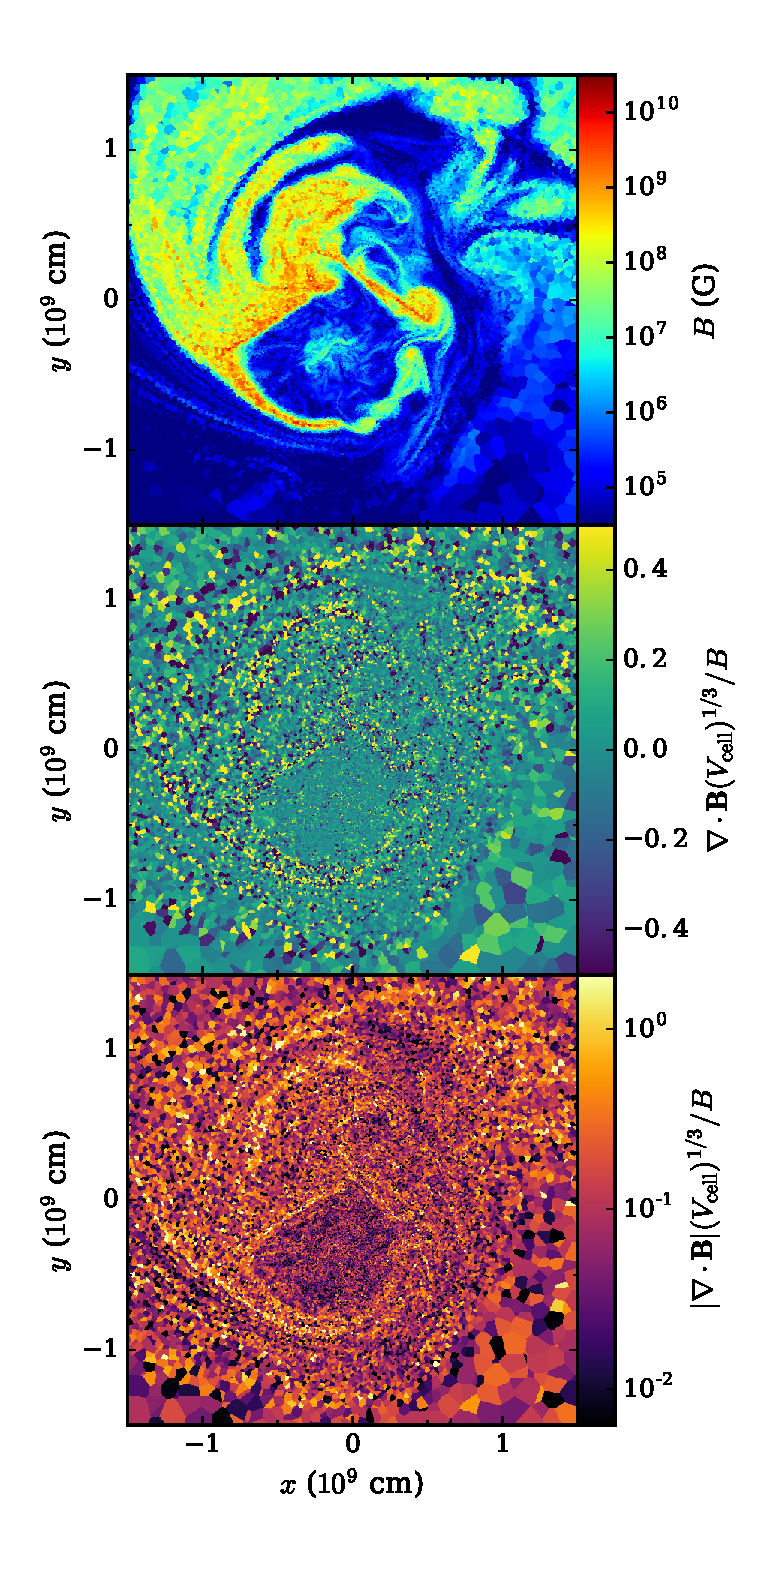
\includegraphics[angle=0,width=0.6\columnwidth]{chapter4_zhu+15/figures/bdiv.pdf}
\caption{From top to bottom, equatorial plane intensity profiles for the magnetic field strength, relative divergence error (linear scale) and absolute relative divergence error (logarithmic) for the simulation at $200\,\mrm{s}$.}
\label{fig:c4_bdiv}
\end{figure}

In Fig. \ref{fig:c4_bdiv}, we show the magnetic field strength, relative divergence error and absolute relative divergence error of our fiducial merger simulation at $t = 200\,\mrm{s}$, when the donor has just been disrupted.  The (mass-weighted) average relative divergence error $\left\langle|\mathbf{\nabla\cdot B}|(V_\mrm{cell})^{1/3}/B\right\rangle = 0.18$ (where $V_\mrm{cell}$ is the Voronoi cell volume), which is typical of both this simulation and \cite{pakms13}'s galaxy disk evolution one, but much larger than typical results from Dedner cleaning-based codes \citep{tric15, hopkr16}.  As in \cite{pakms13}, the divergence error alternates on very small scales (Fig. \ref{fig:c4_bdiv} middle panel), and peaks near large magnetic gradients (comparing top and bottom panels).  While errors cancel over large scales (the average relative error with the sign of the divergence included is $\left\langle\mathbf{\nabla\cdot B}(V_\mrm{cell})^{1/3}/B\right\rangle = -1.4\times10^{-3}$), the regions of highest magnetic gradient correspond to the shear interface between donor and accretor, where we believe the field is amplified.  It is therefore plausible that errors at small scales spuriously magnify the magnetic dynamo associated with the shear layer and Kelvin-Helmholtz vortices.  

This hypothesis is supported by \cite{hopkr16}, who perform a battery of tests comparing the Dedner and Powell mechanisms for their mesh-free finite-volume code \textsc{GIZMO}, and show divergence errors in Powell-based simulations of advection and hydromagnetic instability lead to spurious and unstable field growth.  Moreover, comparisons between Powell and constrained transport-based \arepo\ using simulations of MHD turbulence and disk galaxy evolution show that the Powell scheme leads to greater magnetic field amplification by up to an order of magnitude, as well as a qualitatively different field topology \citep{mocz+16}.

%while \cite{pakms13} find good agreement between Powell-based \arepo\ simulations and CT-based Eulerian ones for the Orzag-Tang vortex problem and magneto-rotational instability within a disk

%In Hopkins's most extreme test, SPH returns divergence errors of order 0.1 - 1 (Gizmo 0.01 - 0.1), but Arepo (pakmor+13) gives errors of order unity!

Caution is therefore in order when using this chapter's results, at least until they have been compared with simulations using \arepo's new constrained transport scheme.  Given that the results will likely be different, it may also be useful to conduct a simpler test case of field evolution within a single Kelvin-Helmholtz vortex at various resolutions and compare the results with those of \cite{oberam10} and \cite{zrakm13}.  Nevertheless, as discussed in Sec. \ref{sec:c4_results}, the remnant magnetic field's bulk properties following coalescence are physically plausible, and are likely to be more robust than the detailed field configuration.  We use these bulk properties (alongside \cite{ji+13}'s work) when considering magnetic simmering WDs the next chapter.

%\cite{pakmv13} find qualitative differences in their resolution test, which they attribute to large divergence errors artificially accelerating magnetic field growth in their low resolution simulations.  While we find no substantial difference in our test, we also check the divergence errors of our two simulations.  We find the time-averaged $\left\langle(\mrm{div} \vec{B}) r/B\right\rangle$ ($\left\langle|\mrm{div} \vec{B}| r/B\right\rangle$ during coalescence only) to be $1.1\times10^{-4}$ ($1.3\times10^{-1}$) for the fiducial run, and $2.0\times10^{-4}$ ($1.4\times10^{-1}$) for the low resolution run.  These errors are comparable to each other, and much smaller than any reported in \cite{pakmv13}.  Divergence errors are spatially highly localized and trace steep magnetic gradients, suggesting that these errors contribute only to small-scale variations in the magnetic field.  \textbf{Editors: $\left\langle(\mrm{div} \vec{B}) r/B\right\rangle$ begins at an enormous $10^{12}$; Ruediger, why would this be?  Did you see something similar in your simulations?}


